\documentclass{beamer}
\usetheme{Dresden}
\usecolortheme{dove}
%% Checking if saving file is working more
%\usepackage{graphicx} %For jpg figure inclusion
%\usepackage{times} %For typeface
%\usepackage{epsfig}
\usepackage{color} %For Comments
\usepackage{beamerthemeshadow} %Paul and Lemmon put this in, take out if you want
%\usepackage[all]{xy}
%\usepackage{float}
%\usepackage{subfigure} 
%\usepackage{hyperref}
%\usepackage{url}
%\usepackage{parskip}
%\usepackage{multirow}

\definecolor{ForestGreen}{RGB}{34,139,34}
\definecolor{BestBlue}{RGB}{80,255,255}
% Uncomment this if you want to show work-in-progress comments
\newcommand{\comment}[1]{{\bf \tt  {#1}}}
% Uncomment this if you don't want to show comments
%\newcommand{\comment}[1]{}
\newcommand{\emcomment}[1]{\textcolor{ForestGreen}{\comment{Elena: {#1}}}}
\newcommand{\todo}[1]{\textcolor{blue}{\comment{To Do: {#1}}}}
\newcommand{\thcomment}[1]{\textcolor{BestBlue}{\comment{Thomas: {#1}}}}
\newcommand{\rmcomment}[1]{\textcolor{magenta}{\comment{Ryan: {#1}}}}
%%%%%%%%%%%%%%%%%%%%%%%%%%%%%%%%%%%%%%%%%%

\begin{document}
\author{Elena Machkasova, Thomas Hagen, Ryan McArthur}
\title{Super-fun with First-class Shapes in Quil}
\date{November 16, 2015}

\begin{frame}
\frametitle {Super-fun with First-class Shapes in Quil}
\maketitle
\end{frame}
%frame

\begin{frame}
\frametitle{Table of contents}
\tableofcontents  
\end{frame}

\section{Who we are and why we are here}

\begin{frame}
\frametitle{Where are we from?}
\begin{figure}[h]
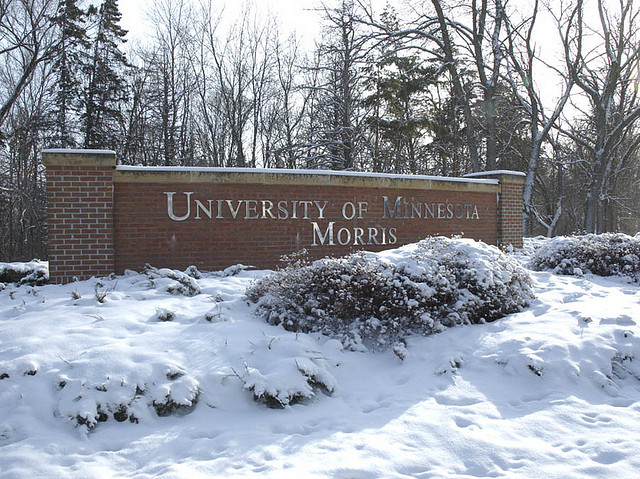
\includegraphics[width=7cm]{PresentationImages/umm-winter.jpg}
\end{figure}
UMM is a small liberal arts campus of UMN located 3 hours driving from Minneaplois/St.Paul. 
\end{frame}

\begin{frame}
\frametitle{What are we working on?}
Developing Clojure-based introductory CS course ({\it \href{http://cda.morris.umn.edu/~elenam/\#clojure}{ClojurEd project}}). 

What does this include? 
\begin{enumerate}
\item Beginner-friendly error messages. 
\item Libraries and tools 
\end{enumerate}
\end{frame}

\begin{frame}
\frametitle{Odds and ends (not an actual slide)}
\emcomment{Don't forget:
\begin{enumerate}
\item Mention Racket influence  
\item Mention the author Quil fun mode
\item Mention Tom Hall EuroClojure 2014
\end{enumerate}
}
\end{frame}

\begin{frame}
	\frametitle{Future Work}
	\begin{itemize}
		\item Fill out more functionality
		\begin{itemize}
			\item Rotate more complex shapes
			\item Pixel-detail Overlay and Overlay-Align
			\item More seemless integration with Quil fun-mode
		\end{itemize}
		\item Open Source the project \emcomment{Done?}
		\item Integrate a Clojure sound library
	\end{itemize}
\end{frame}

\begin{frame}
\frametitle{Acknowledgments}
\emcomment{Need proper acknowledgments and logos; also probably thank Cognitect and other conj sponsors for providing an opportunity to talk}
	Our research was sponsored by:
	\begin{itemize}
	\item HHMI
	\item LSAMP
	\end{itemize}
	{\centering
	\noindent
	Thank you! \par
	Any questions? \par
	}
\end{frame}
\end{document}
